\chapter{Introduction}

\section{Motivation \& Problem Statement}

Parsing of programming languages is an often studied and revered technique in the computer sciences. The same is not true for configuration file parsing. The answer to the question “How do I solve this problem?” does usually not contain the task of creating and parsing a new programming language in the process. On the other hand, the answer to “How do I configure this?” often seems to be thinking about a new configuration file format and then implementing handwritten parser code for it.

While hand written parsing code can be the proper tool to convert code, for example both \href{http://clang.llvm.org}{Clang}~\cite{bendersky2012clang} and \href{http://gcc.gnu.org}{GCC}~\cite{myers2008cparser} use handwritten parsers, often the person writing configuration parsing code is not an expert in parsing. As consequence, configuration file parsers often suffer from problems such as

\begin{itemize}
  \item bad or no error message support,
  \item no error recovery, and
  \item no proper encoding support.
\end{itemize}

One of the reasons for these problems is that computer programmers usually think of configuration file parsing as easy and not that important. After all, misconfiguration is also often seen as a problem of the user and not of the application~\cite{xu2013not}.

In this thesis we will look at the configuration file parsing problem and evaluate different options to convert configuration settings. Notable examples include:

\begin{itemize}
  \item bidirectional programming~\cite{foster2005combinators, bohannon2006relational, lutterkort2008augeas, ko2016bigul, raab2016improving},
  \item code produced by a parser generator~\cite{denny2008ielr, parr2014adaptive, warth2016modular, bates2017aprt},
  \item serialization libraries~\cite{sumaray2012cds, pacini2015performance}, and
  \item hand-written parsers~\cite{myers2008cparser, bendersky2012clang}
\end{itemize}

. Currently the possibilities to compare different parsing techniques are limited. The naïve approach would be to just run different parsers on the same data. In practice however, this approach is not usable, since parser tools tend to produce very different data structures. Some of them do not produce data structures at all, instead they let the user specify subroutines that should be called when the parser matches parts of the grammar.

\begin{figure}[H]
  \centering
    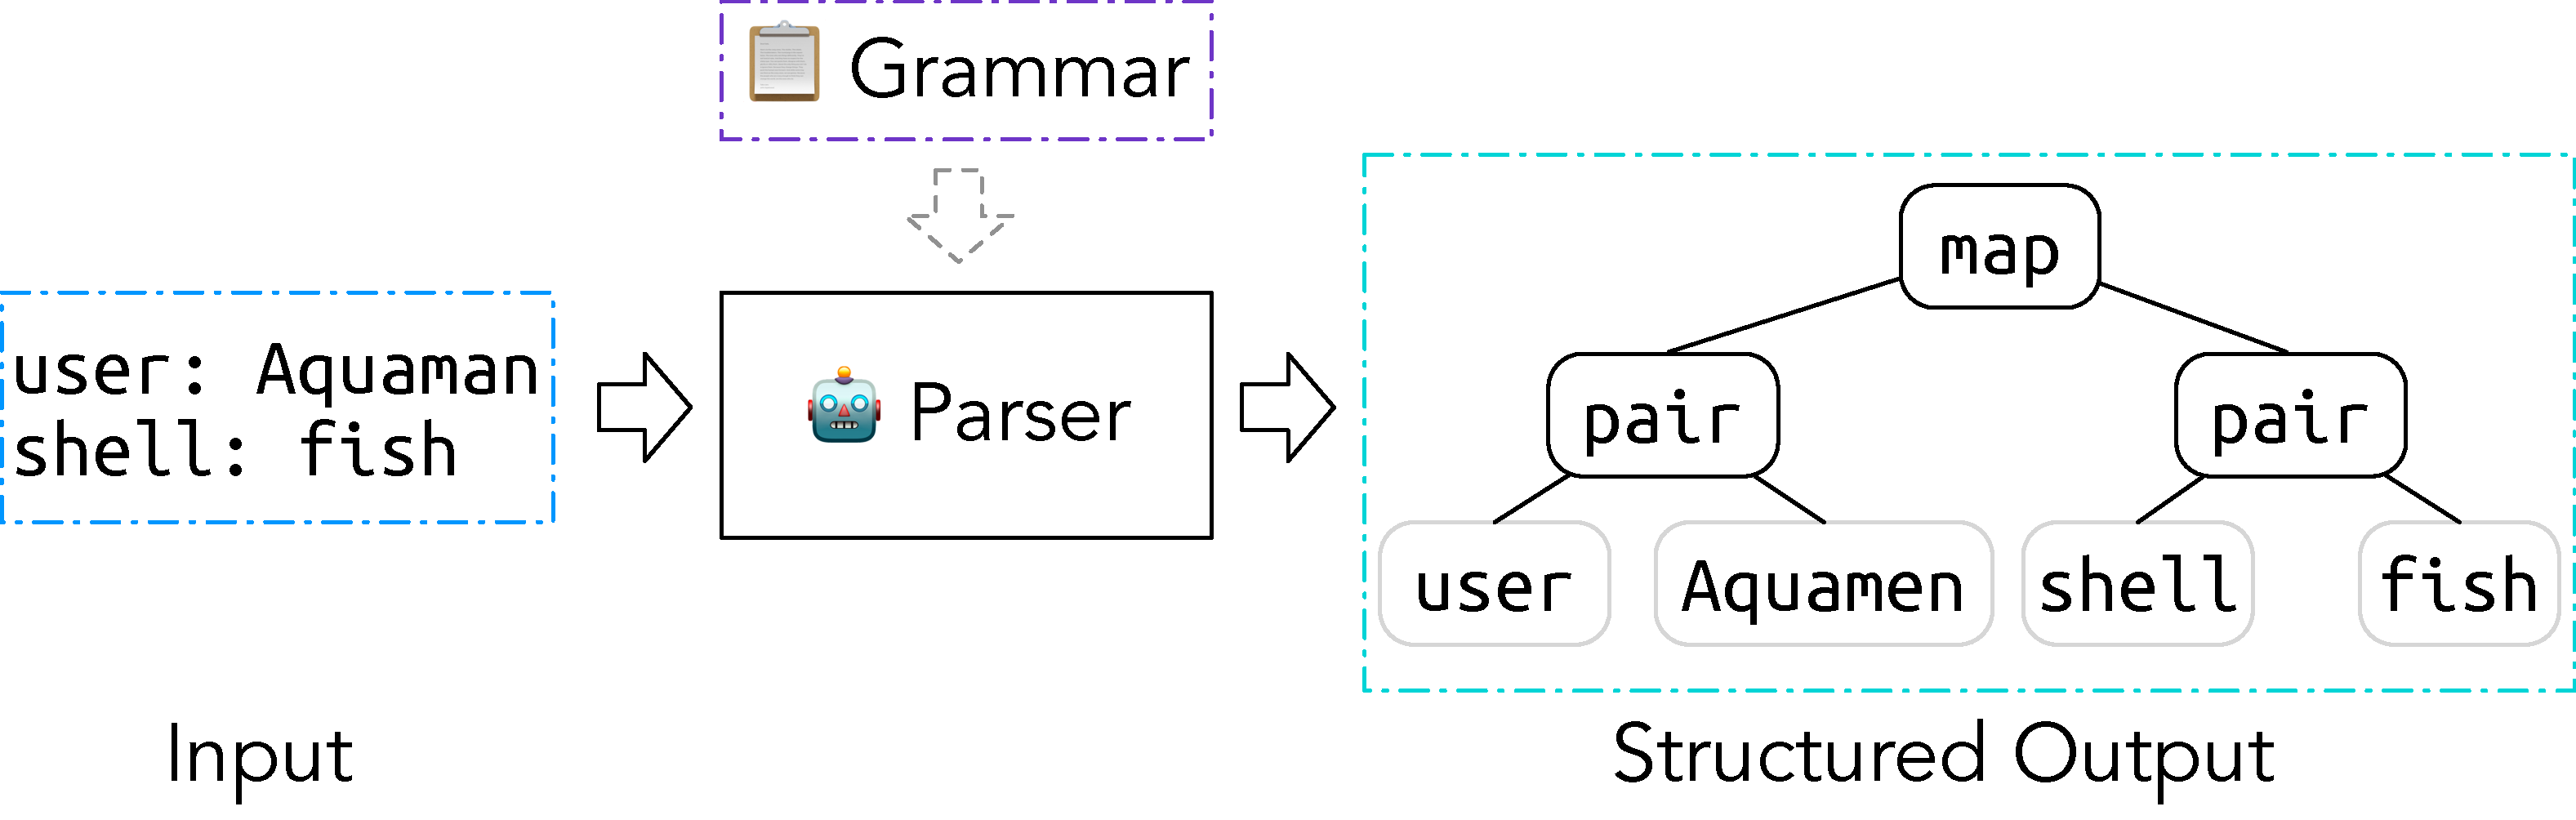
\includegraphics[width=\textwidth]{Parsing}
  \caption{Simplified view of a parsing process}
\end{figure}

As part of this thesis we will tackle this problem, using different parsing techniques within a common configuration framework. This integration eliminates the problem of comparing the parsing process under different circumstances, since the data structures the parsers create will always be the same. We will use \href{https://libelektra.org}{Elektra}, a key-value database, as configuration framework. Elektra’s storage plugin interface will act as foundation for the parsing process. In the end the thesis should provide answers about which parsing techniques provide an ideal balance between performance and usability.

\section{Aim of the Work}
\label{sec:aim_of_the_work}

Elektra~\cite{raab2010modular, raab2017context} is a plugin-based framework that stores configuration parameters in a \gls{KDB}. Elektra reads and stores configuration data via so-called \emph{storage plugins}.

\begin{figure}[H]
  \centering
    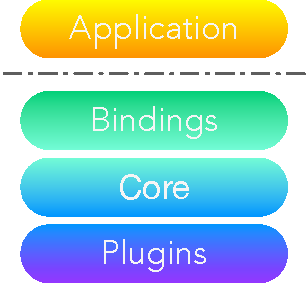
\includegraphics[width=.3\textwidth]{Elektra}
  \caption{The diagram above shows an architecture overview of Elektra. Plugins, are among other things, responsible for parsing and writing configuration data. The core is written in C and provides a low level \gls{API} to access configuration settings. Bindings provide higher-level access to configuration data in C and other languages, such as Java, Lua, Python and Ruby.}
\end{figure}

As part of this thesis we compare various ways of parsing. For that purpose we wrote and generated parsing code for different storage plugins. All of these storage plugins parse a minimal subset of \glstext{YAML}, a human readable language used to specify data. We looked at the following state of the art parsing technologies:

\begin{itemize}
  \item handwritten recursive descent parser (\href{https://github.com/jbeder/yaml-cpp}{yaml-cpp}),
  \item \glstext{ALL(*)} parser generator (\href{http://www.antlr.org}{ANTLR}),
  \item LR parser generator (\href{https://www.gnu.org/software/bison}{Bison}),
  \item Earley parser (\href{https://github.com/vnmakarov/yaep}{YAEP}),
  \item \glstext{PEG} parser (\href{https://github.com/taocpp/PEGTL}{PEGTL}),
  \item parser combinator (\href{https://github.com/orangeduck/mpc}{mpc}), and
  \item bidirectional programming (\href{http://augeas.net}{Augeas})
\end{itemize}

. We compare the parsing code according to the following criteria:

\begin{itemize}
  \item runtime performance,
  \item memory usage,
  \item code size,
  \item overall code complexity,
  \item ease of extensibility and composability, and
  \item error reporting
\end{itemize}

. In the scope of the above comparison we answer the questions below.

\begin{restatable}{question}{speed}
  \label{que:speed}
  How does the theoretic runtime complexity of the parsing methods compare to the actual measured runtime of the parsing code?
\end{restatable}

\begin{restatable}{question}{closeness}
  \label{que:closeness}
  Which parsing technique allows us to stay closest to the definition of the configuration language? Does staying close to the given definition
  allow us to extend and improve the parser and its support code more easily?
\end{restatable}

\section{Methodological Approach}

The methodological approach for this thesis consists of the steps given below.

\begin{description}[style=multiline, leftmargin=3.2cm, font=\bfseries]

  \item[Literature Review] We determined the current status of parsing techniques suitable for configuration file parsing. We then chose appropriate libraries for the parsing techniques listed in the section “\nameref{sec:aim_of_the_work}”.

  \item[Discussion] To determine a minimal usable subset of \glstext{YAML} we decided about common features required for a new Elektra storage plugin with some of the current developers. For that purpose we presented YAML features and asked, which ones should be supported in a survey.

  \item[Implementation] We wrote parsing code that handles our minimal \glstext{YAML} subset. In this phase we also added other necessary support code to Elektra.

  \item[Comparison] As noted in “\nameref{sec:aim_of_the_work}” we evaluated the different implementations of our minimal \glstext{YAML} subset parsers.

  \begin{description}
    \item[Runtime Benchmark:] For the runtime comparison we created a benchmark framework to determine the speed of the different parsing code. In this part of the thesis, we answer \Cref{que:speed}.

    \item[Memory Profiling:] For the memory comparison we use a memory profiling tool to determine the heap memory usage of the \glstext{YAML} plugins.

    \item[Code Count:] We counted the number of code lines with a code line counting tool. This method allow us to consider only actual code, ignoring blank lines and comments.

    \item[Complexity Measurement:] We measured the \gls{CC} of the code using a static analyzer.

    \item[Extensibility \& Composability Check:] To analyze the extensibility and composability of the parsing code we looked at the code difference of commits for certain features and bug fixes. We counted the amount of updated code lines to determine the extension effort. This measurement, together with a comparison between the grammar specification of \glstext{YAML} and the code created in this thesis, helps us to determine the answer for \Cref{que:closeness}.

    \item[Error Reporting:] To determine the quality of the error messages we created erroneous files and compared the quality of the resulting error output.
  \end{description}

\end{description}

\section{Contributions}

\begin{itemize}[style=multiline, leftmargin=3cm, font=\bfseries]
  \item[Parsing Engine Integration] We added plugins for four general purpose parsing engines (\glstext{ANTLR}, Bison, \glstext{YAEP}, \glstext{PEGTL}) to the Elektra framework. These plugins parse a subset of YAML, and can be adapted to parse other configuration languages.

  \item[Benchmark Framework] We created a parser benchmark framework. This framework compares configuration parsers under fair circumstances, since we require and verify that the parsers produce the same data for the same YAML input.

  \item[Support Plugins] In this work we
  \begin{itemize}
    \item created a plugin that add full support for mapping node-based configurations formats, such as JSON and YAML, to Elektra’s data structures,
    \item extended a plugin to convert Base64 encoded YAML data into binary Elektra data, and
    \item created a plugin that deserializes Elektra’s data structures into YAML data.
  \end{itemize}

  \item[\gls{FLOSS} Contributions] During the work of this thesis the author

  \begin{itemize}
    \item reported \href{https://github.com/ElektraInitiative/libelektra/issues/created_by/sanssecours}{over 100 problems in Elektra’s issue tracker},
    \item \href{https://github.com/ElektraInitiative/libelektra/pulls?q=is%3Apr+is%3Aopen+reviewed-by%3Asanssecours}{reviewed over 80 pull requests},
    \item \href{https://github.com/ElektraInitiative/libelektra/graphs/contributors?from=2012-04-01&to=2019-09-30&type=c}{committed over 3 800 times} to Elektra,
    \item opened \href{https://github.com/ElektraInitiative/libelektra/pulls?q=is%3Apr+is%3Amerged+author%3Asanssecours}{over 360 merged pull requests}, and
    \item \href{https://github.com/ElektraInitiative/libelektra/graphs/contributors?from=2012-04-01&to=2019-09-30&type=a}{added over 100 000 lines} to, and \href{https://github.com/ElektraInitiative/libelektra/graphs/contributors?from=2012-04-01&to=2019-09-30&type=d}{removed over 100 000 lines} from Elektra’s code base.
  \end{itemize}
\end{itemize}

\section{Structure of this Thesis}

In chapter~\ref{sec:background} we provide background information about the state of art in configuration file parsing. We then describe the configuration framework Elektra, and give some examples about other parser comparison related research.

In chapter~\ref{sec:design_challenges_and_decisions} we describe the design challenges we faced and the decisions we made when we implemented the parer plugins. First we describe how we decided about the YAML subset the parsers should be able to parse. Then we explain how we mapped YAML data into the data structures of Elektra. After that we discuss the problems we had when we implemented the plugins and how we solved them. At the end of the chapter we talk about the additional Elektra plugins we wrote to improve the integration of the parser plugins into Elektra.

Chapter~\ref{sec:evaluation} provides a detailed evaluation of the parsers. It first describes the goals of the evaluation, detailing different important criteria of the parser plugins. Afterwards we analyze each of the criteria in their own section, answering our research questions in the process. At the end of the evaluation we describe the parser plugins that best fit our criteria.

In chapter~\ref{sec:conclusion_and_future_work} we conclude the the thesis with an overview of the results and describe possible future work.
